\subsection{Backend Modultest}

Dette afsnit omhandler modultesten af backenden, denne deles op i følgende to dele, der fortages først en modultest af DAL som kan findes her \autoref{ssec: Modultest database} , hvorefter DAL bruges i modultesten af Web api’et, da Web api’et ikke vil blive testet uden DAL modulet.\\

Til at udføre modultests af web api’et benyttes udviklingsværktøjet Swashbuckle \cite{Swagger}. Swashbuckle bruges til at bygge SwaggerDocument objekter på baggrund af de routes, controllers og modeller som er blevet udviklet. Hertil tilbyder Swashbuckle et Swagger User interface, hvor man kan teste sine http funktioner og se om man modtager den forventede response. Derfor er dette et oplagt værktøj at gøre brug af. Et billede af Swagger User interfacet kan ses på \autoref{fig:Modultest-Backend-swagger}.\\

\begin{figure}[H]
\centering
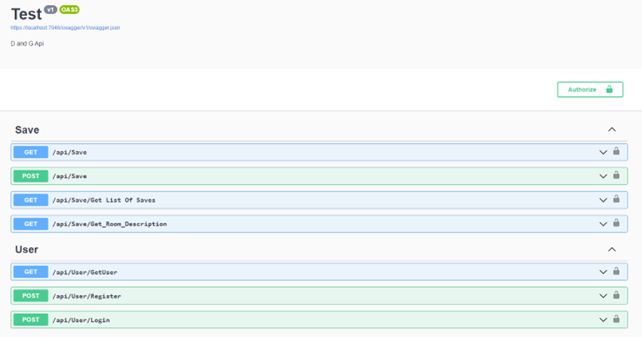
\includegraphics[width = \textwidth]{02-Body/Images/Backend_swagger.PNG}
\caption{Swagger User interface, som viser de forskellige http metoder}
\label{fig:Modultest-Backend-swagger}
\end{figure}

For at aktivere swagger tilføjes følgende middleware til program.cs AddSwaggerGen(), UseSwagger() og UseSwaggerUI(). Til SwaggerGen tilføjes også security med JWT tokens så Authentication og Authorization kan testes.\\

I \autoref{table: succes} kan ses en tabel oversigt over tests af succes scenarie, for de enkelte funktioner samt resultater.\\


\begin{table}[H]
\caption{Tabel over modultest af Backendes Web Api, her vises testes af succes scenarier for alle Web Api http funktioner }%
\label{table: succes}
\begin{tabular}{|p{0.75cm}|p{3.6cm}|p{3.5cm}|p{3.5cm}|p{1.9cm}|} \hline
 \textbf{Test} & \textbf{Funktion} & \textbf{Forventet resultat} & \textbf{Observering} & \textbf{Vurdering} \textbf{(OK/Fail)}\\\hline
 1 & PostSave(SaveDTO saveDTO) & Der bliver sendt et specifikt gamestate, for brugeren der er logget ind. & Det er muligt at sende game statet, og de korrekte værdier bliver sendt med. & OK \\ \hline
 2 & Register(UserDTO regUser) & Der registreres en ny bruger, ved at gemme oplysninger omkring denne. Der returneres en JWT-token. & Brugeren bliver registreret, og kan findes blandt de andre brugere. Det ses at der returneres en JWT-token. & OK \\ \hline
 3 & Login(UserDTO userDTO) & Der tjekkes om oplysningerne passer med en registreret bruger, og passer det logges der ind. Der returneres en JWT-token. & Det lykkedes at logge ind, og der returneres en JWT-token.  & OK \\ \hline
 4 & GetSave(int id) & Der hentes et specifikt save for den bruger der er logget ind. & Det lykkedes at hente et specifikt game state, uden errors  & OK \\ \hline
 5 & GetListOfSave() & Der hentes en liste af game states, for brugeren der er logget ind. & Det lykkedes at hente en liste af game states, for den specifikke bruger. & OK \\ \hline
 6 & GetRoomDescription(int id) & Denne route henter en beskrivelse af det valgt rum i spillet. & Det ses, at der bliver hentet en beskrivelse af det valgte rum. & OK \\ \hline
\end{tabular}
\end{table}

I nedenstående tabel \label{table: fejl} testes om funktionerne håndtere fejlscenarier korrekt.

\begin{table}[H]
\caption{Tabel over modultest af Backendes Web Api, her vises testes af fejlscenarier for alle Web Api http funktioner}%
\label{table: fejl}
\begin{tabular}{|p{0.75cm}|p{3.6cm}|p{3.5cm}|p{3.5cm}|p{1.9cm}|} \hline
 \textbf{Test} & \textbf{Funktion} & \textbf{Forventet resultat} & \textbf{Observering} & \textbf{Vurdering} \textbf{(OK/Fail)}\\\hline
 1 & Register(UserDTO regUser) & Brugernavnet er allerede i brug, og der sendes en fejlmeddelelse  & Status: 400. Besked: ”Name is already in use”. & OK \\ \hline
 2 & Login(UserDTO userDTO) & Oplysningerne stemmer ikke overens med en registreret bruger, og der bør sendes en fejlmeddelelse. & Status: 400. Besked: ”Wrong Username or Password” & OK \\ \hline
 3 & GetSave(int id) & Der er ikke logget ind, så der kan ikke hentes et game state. & Status: 401, Unauthorized & OK \\ \hline
 4 & GetListOfSave() & Der er ikke logget ind, og derfor kan der ikke hentes et liste. &Status: 401, Unauthorized  & OK \\ \hline
 5 & PostSave(SaveDTO saveDTO) & Der er ikke logget ind, og derfor kan der ikke gemmes er spil. & Status: 401, Unauthorized & OK \\ \hline

\end{tabular}
\end{table}

Med alle funktioner testet med et godkendt resultat, er backenden klar til at blive integreret med de andre moduler for systemet.



\newpage
